% ****** Start of file apssamp.tex ******
%
%   This file is part of the APS files in the REVTeX 4.2 distribution.
%   Version 4.2a of REVTeX, December 2014
%
%   Copyright (c) 2014 The American Physical Society.
%
%   See the REVTeX 4 README file for restrictions and more information.
%
% TeX'ing this file requires that you have AMS-LaTeX 2.0 installed
% as well as the rest of the prerequisites for REVTeX 4.2
%
% See the REVTeX 4 README file
% It also requires running BibTeX. The commands are as follows:
%
%  1)  latex apssamp.tex
%  2)  bibtex apssamp
%  3)  latex apssamp.tex
%  4)  latex apssamp.tex
%
\documentclass[%
 reprint,
%superscriptaddress,
%groupedaddress,
%unsortedaddress,
%runinaddress,
%frontmatterverbose, 
%preprint,
%preprintnumbers,
%nofootinbib,
%nobibnotes,
%bibnotes,
 amsmath,amssymb,
 aps,
%pra,
%prb,
%rmp,
%prstab,
%prstper,
%floatfix,
]{revtex4-2}

\usepackage{graphicx}% Include figure files
\usepackage{dcolumn}% Align table columns on decimal point
\usepackage{bm}% bold math
\usepackage{array}
\usepackage{url}% format URLs in bibliography
%\usepackage{hyperref}% add hypertext capabilities
%\usepackage[mathlines]{lineno}% Enable numbering of text and display math
%\linenumbers\relax % Commence numbering lines

%\usepackage[showframe,%Uncomment any one of the following lines to test 
%%scale=0.7, marginratio={1:1, 2:3}, ignoreall,% default settings
%%text={7in,10in},centering,
%%margin=1.5in,
%%total={6.5in,8.75in}, top=1.2in, left=0.9in, includefoot,
%%height=10in,a5paper,hmargin={3cm,0.8in},
%]{geometry}




\begin{document}


\title{Determination of the Elementary Charge via Computer-Vision-Assisted Millikan Oil Drop Experiment}

\author{Kevin A. Acosta}
\author{Kevin J. Medina}
\author{Natalie Muñoz-Melesio}

\begin{abstract}
We replicate Millikan's oil drop experiment~\cite{Millikan1913} using the PASCO AP-8210A apparatus~\cite{PASCO-AP8210A} and automated computer vision tracking to determine the elementary charge \(q_e\). Charged oil droplets were recorded via webcam across four trial videos; a detection and tracking algorithm extracted rise and fall velocities for each droplet. After applying validity criteria (1--20 electrons, \textless 50\% relative error), 141 measurements yielded \(q_e = (1.608 \pm 0.005) \times 10^{-19}\)~C, a +0.38\% deviation from the accepted value~\cite{NIST-e-2022}. A Monte Carlo simulation validated the analysis procedure, recovering the input charge to within 0.03\%. The broad distribution of integer electron counts ($n = 2$ to $20$) confirms charge quantization.
\end{abstract}


\maketitle


\section{Introduction}

In 1913, Robert A. Millikan measured the charge of individual oil droplets suspended in an electric field and showed that electric charge comes in discrete, integer multiples of a fundamental unit~\cite{Millikan1913}. This direct evidence for charge quantization earned him the 1923 Nobel Prize in Physics and remains one of the most replicated experiments in physics education~\cite{Franklin1997}. The accepted value of the elementary charge is now known to extraordinary precision, $e = 1.602\,176\,634 \times 10^{-19}$~C, as established by the 2022 CODATA adjustment~\cite{NIST-e-2022}. However, the traditional manual approach---timing a single droplet with a stopwatch while watching through a microscope---is tedious, limited to a handful of measurements per session, and susceptible to observer bias~\cite{Heering2010}. In this work, we replace manual timing with automated computer vision tracking applied to webcam video of the PASCO AP-8210A apparatus~\cite{PASCO-AP8210A}, yielding over two orders of magnitude more measurements than the manual method. The charge on each droplet is determined by balancing gravitational, viscous, and electrostatic forces~\cite{Griffiths2017}, following the analysis procedure in the PASCO manual~\cite{PASCO-AP8210A}. Because each droplet carries an unknown integer number of elementary charges, the value of \(q_e\) is inferred by dividing measured total charges by the nearest integer.

We also developed a Monte Carlo simulation of the experiment to validate our analysis pipeline before applying it to real data. By generating synthetic droplet velocities with known input charges and adding controlled Gaussian noise, we confirmed that the analysis correctly recovers \(q_e\) and that the error propagation yields realistic uncertainties.

\section{Methods}

\subsection{Theory}

The elementary charge is calculated using the Millikan formula from the PASCO AP-8210A manual~\cite{PASCO-AP8210A}. At terminal fall velocity, the gravitational force on a droplet equals the viscous drag. The Cunningham slip correction is necessary because the droplet radii in this experiment (0.5--1.6~$\mu$m) approach the mean free path of air molecules ($\sim$0.07~$\mu$m), a regime where the continuum assumption underlying Stokes' law~\cite{Stokes1851} breaks down and the effective viscous drag is reduced~\cite{Cunningham1910}. Using Stokes' law with the Cunningham slip correction for sub-micron particles, the droplet radius is:

\begin{equation}
    a = \sqrt{\left(\frac{b}{2p}\right)^{2} + \frac{9 \eta v_f}{2 g \rho}} - \frac{b}{2p}
\end{equation}

where $b = 8.20 \times 10^{-3}$~Pa$\cdot$m is the Cunningham correction constant and $p$ is the atmospheric pressure. With the electric field applied, a charged droplet at terminal rise velocity satisfies the force balance $qE = mg(v_f + v_r)/v_f$, yielding the charge:

\begin{equation}
    q = \frac{4}{3} \pi \rho g\, a^{3} \frac{(v_f + v_r)}{E\, v_f}
\end{equation}

where $E = V/d$ is the electric field strength. The integer number of elementary charges is determined by $n = \text{round}(q / e_{\text{accepted}})$, and the per-measurement estimate is $e_{\text{calc}} = q / n$.

The experimental parameters and their uncertainties are:
\begin{itemize}
\item $d = (7.5 \pm 0.1) \times 10^{-3}$~m -- plate separation (measured with micrometer)
\item $V = 500 \pm 0.1$~V -- plate voltage (measured with digital multimeter)
\item $\rho = 886 \pm 5$~kg/m$^3$ -- oil density (Squibb \#5597 Mineral Oil)
\item $\eta = (1.813 \pm 0.004) \times 10^{-5}$~N$\cdot$s/m$^2$ -- air viscosity at 20$^\circ$C
\item $b = (8.20 \pm 0.08) \times 10^{-3}$~Pa$\cdot$m -- Cunningham correction constant
\item $p = 101{,}325 \pm 1{,}000$~Pa -- atmospheric pressure
\end{itemize}
\subsection{Physical Experiment}
\subsubsection{Environmental Setup}
The experiment was conducted in a darkened room with a dark background behind the apparatus. The apparatus was positioned on a stable surface free from drafts and vibrations, and leveled using the built-in bubble level, as environmental disturbances can interfere with droplet velocity measurements. Figure~\ref{fig:setup} shows the experimental apparatus with the webcam positioned at the eyepiece.

\begin{figure}[h]
\centering
\includegraphics[width=\columnwidth]{IMG_2855.png}
\caption{Photograph of the PASCO AP-8210A Millikan Oil Drop Apparatus used in this experiment. The webcam (right) is mounted at the eyepiece of the viewing scope. The high-voltage DC power supply connects to the parallel-plate capacitor inside the droplet viewing chamber. The atomizer (top left) introduces charged oil droplets into the chamber through a small hole in the lid.}
\label{fig:setup}
\end{figure}

\subsubsection{Measuring Plate Separation}
The thickness of the plastic spacer plate was measured with a micrometer, excluding the raised rim, yielding a plate separation of $d = 7.5 \pm 0.1$~mm.

\subsubsection{Adjusting and Measuring Voltage}
The high-voltage DC power supply was set to 500~V, and the actual voltage delivered to the plate connectors was verified with a digital multimeter. The measured voltage was $V = 500 \pm 0.1$~V.

\subsubsection{Determining the Temperature of the Droplet Viewing Chamber}
The temperature inside the droplet viewing chamber was determined from the thermistor resistance table on the apparatus platform. The chamber temperature was approximately 20$^\circ$C, corresponding to an air viscosity of $\eta = 1.813 \times 10^{-5}$~N$\cdot$s/m$^2$ from the PASCO manual Appendix~A~\cite{PASCO-AP8210A}.

\subsubsection{Introducing the Droplets Into the Chamber}
The atomizer was filled with Squibb \#5597 non-volatile mineral oil (density 886~kg/m$^3$). The ionization source lever was moved to the ``Spray Droplet Position'' to allow air to escape from the chamber during droplet introduction. The atomizer tip was inserted into the hole on the lid of the droplet viewing chamber, and the bulb was squeezed once while observing through the viewing scope. Once a shower of droplets became visible, the ionization source lever was returned to the ``OFF'' position. It is worth noting that the droplet hole cover as described in the PASCO manual was not available. Instead, after dispensing the oil, the hole in the lid of the droplet viewing chamber was covered with tape, preventing air movement from disturbing the droplets in the chamber, which was previously causing excessive lateral movement in the droplets, preventing extended observation.

\subsubsection{Recording Droplet Dynamics}
A webcam was used to record video of the droplets visible through the viewing scope. The webcam captured droplets falling under gravity, then the plate polarity was switched to record droplets rising under the electric field. This procedure was repeated across four trials. For selected trials, the ionization source lever was moved to the ``ON'' position to expose droplets to alpha particles from the thorium-232 source, altering their charge state before additional rise and fall recordings. The plate potential, oil density, air viscosity at the chamber temperature, and barometric pressure were recorded for each trial.

\subsubsection{Performing Data Collection}

Four trial videos totalling approximately 31,940 frames ($\sim$18 minutes of footage at 30fps) were recorded using a webcam placed at the eyepiece of the PASCO Oil Drop Apparatus.
Oil droplets appear as bright points against the dark background of the Millikan apparatus viewing chamber. The detection algorithm employs local mean subtraction to identify these bright spots. For each video frame, the algorithm applies Gaussian smoothing (5$\times$5 kernel) to reduce sensor noise, then subtracts a local background estimate (51$\times$51 pixel averaging window) from the smoothed image, producing a difference map where droplets appear as positive peaks. Binary thresholding (threshold = 10 intensity units above local mean) is applied to isolate candidate droplets, followed by morphological opening and closing (3$\times$3 kernel) to remove noise and fill small gaps. Connected component analysis identifies individual droplet regions, measuring centroid positions, areas, and brightness values. Components are filtered based on area (4--350~px$^2$) and minimum brightness (75 intensity units) to reject noise, dust particles, and out-of-focus objects.


Frame-to-frame tracking associates detected droplets across time using a nearest-neighbor algorithm with motion prediction. For each existing track, the algorithm predicts the droplet's next position based on its recent velocity history. Detected droplets are matched to tracks if they fall within a maximum distance threshold of 10 pixels per elapsed frame of the predicted position, enabling robust tracking even when droplets temporarily overlap or briefly disappear. The tracking system maintains continuity through brief detection gaps (up to 3 frames) by extrapolating predicted positions. Unmatched new detections initiate new tracks, while tracks that remain unmatched beyond the gap tolerance are terminated. This approach balances sensitivity against false track termination or fragmentation.


The algorithm segments each track into distinct rise/fall phases by analyzing the sign of vertical velocity. Consecutive frames with consistent downward motion are grouped into fall segments, while upward motion constitutes rise segments. To ensure statistical reliability, we require minimum segment durations of 8 frames and minimum total track lengths of 30 frames. Velocities are computed from position differences and frame timestamps, with the median velocity used per segment for robustness against outliers. Only tracks exhibiting both fall and rise segments are retained for analysis.


The detection and tracking algorithms contain adjustable parameters that affect the tradeoff between data quantity and quality. A systematic parameter sensitivity sweep was performed, evaluating six named configurations against two criteria: (1) maximizing the number of valid measurements, and (2) minimizing the deviation from the accepted elementary charge value. A measurement was deemed valid if the calculated charge corresponded to 1--20 elementary charges with individual error below 50\%. The optimized parameters (detection threshold = 10, area range = 4--350~px$^2$, minimum brightness = 75, maximum tracking distance = 10~px/frame, gap tolerance = 3 frames, minimum segment length = 8 frames, minimum track length = 30 frames) maximize data yield while maintaining sub-1\% overall error.


\begin{figure}[h]
\centering
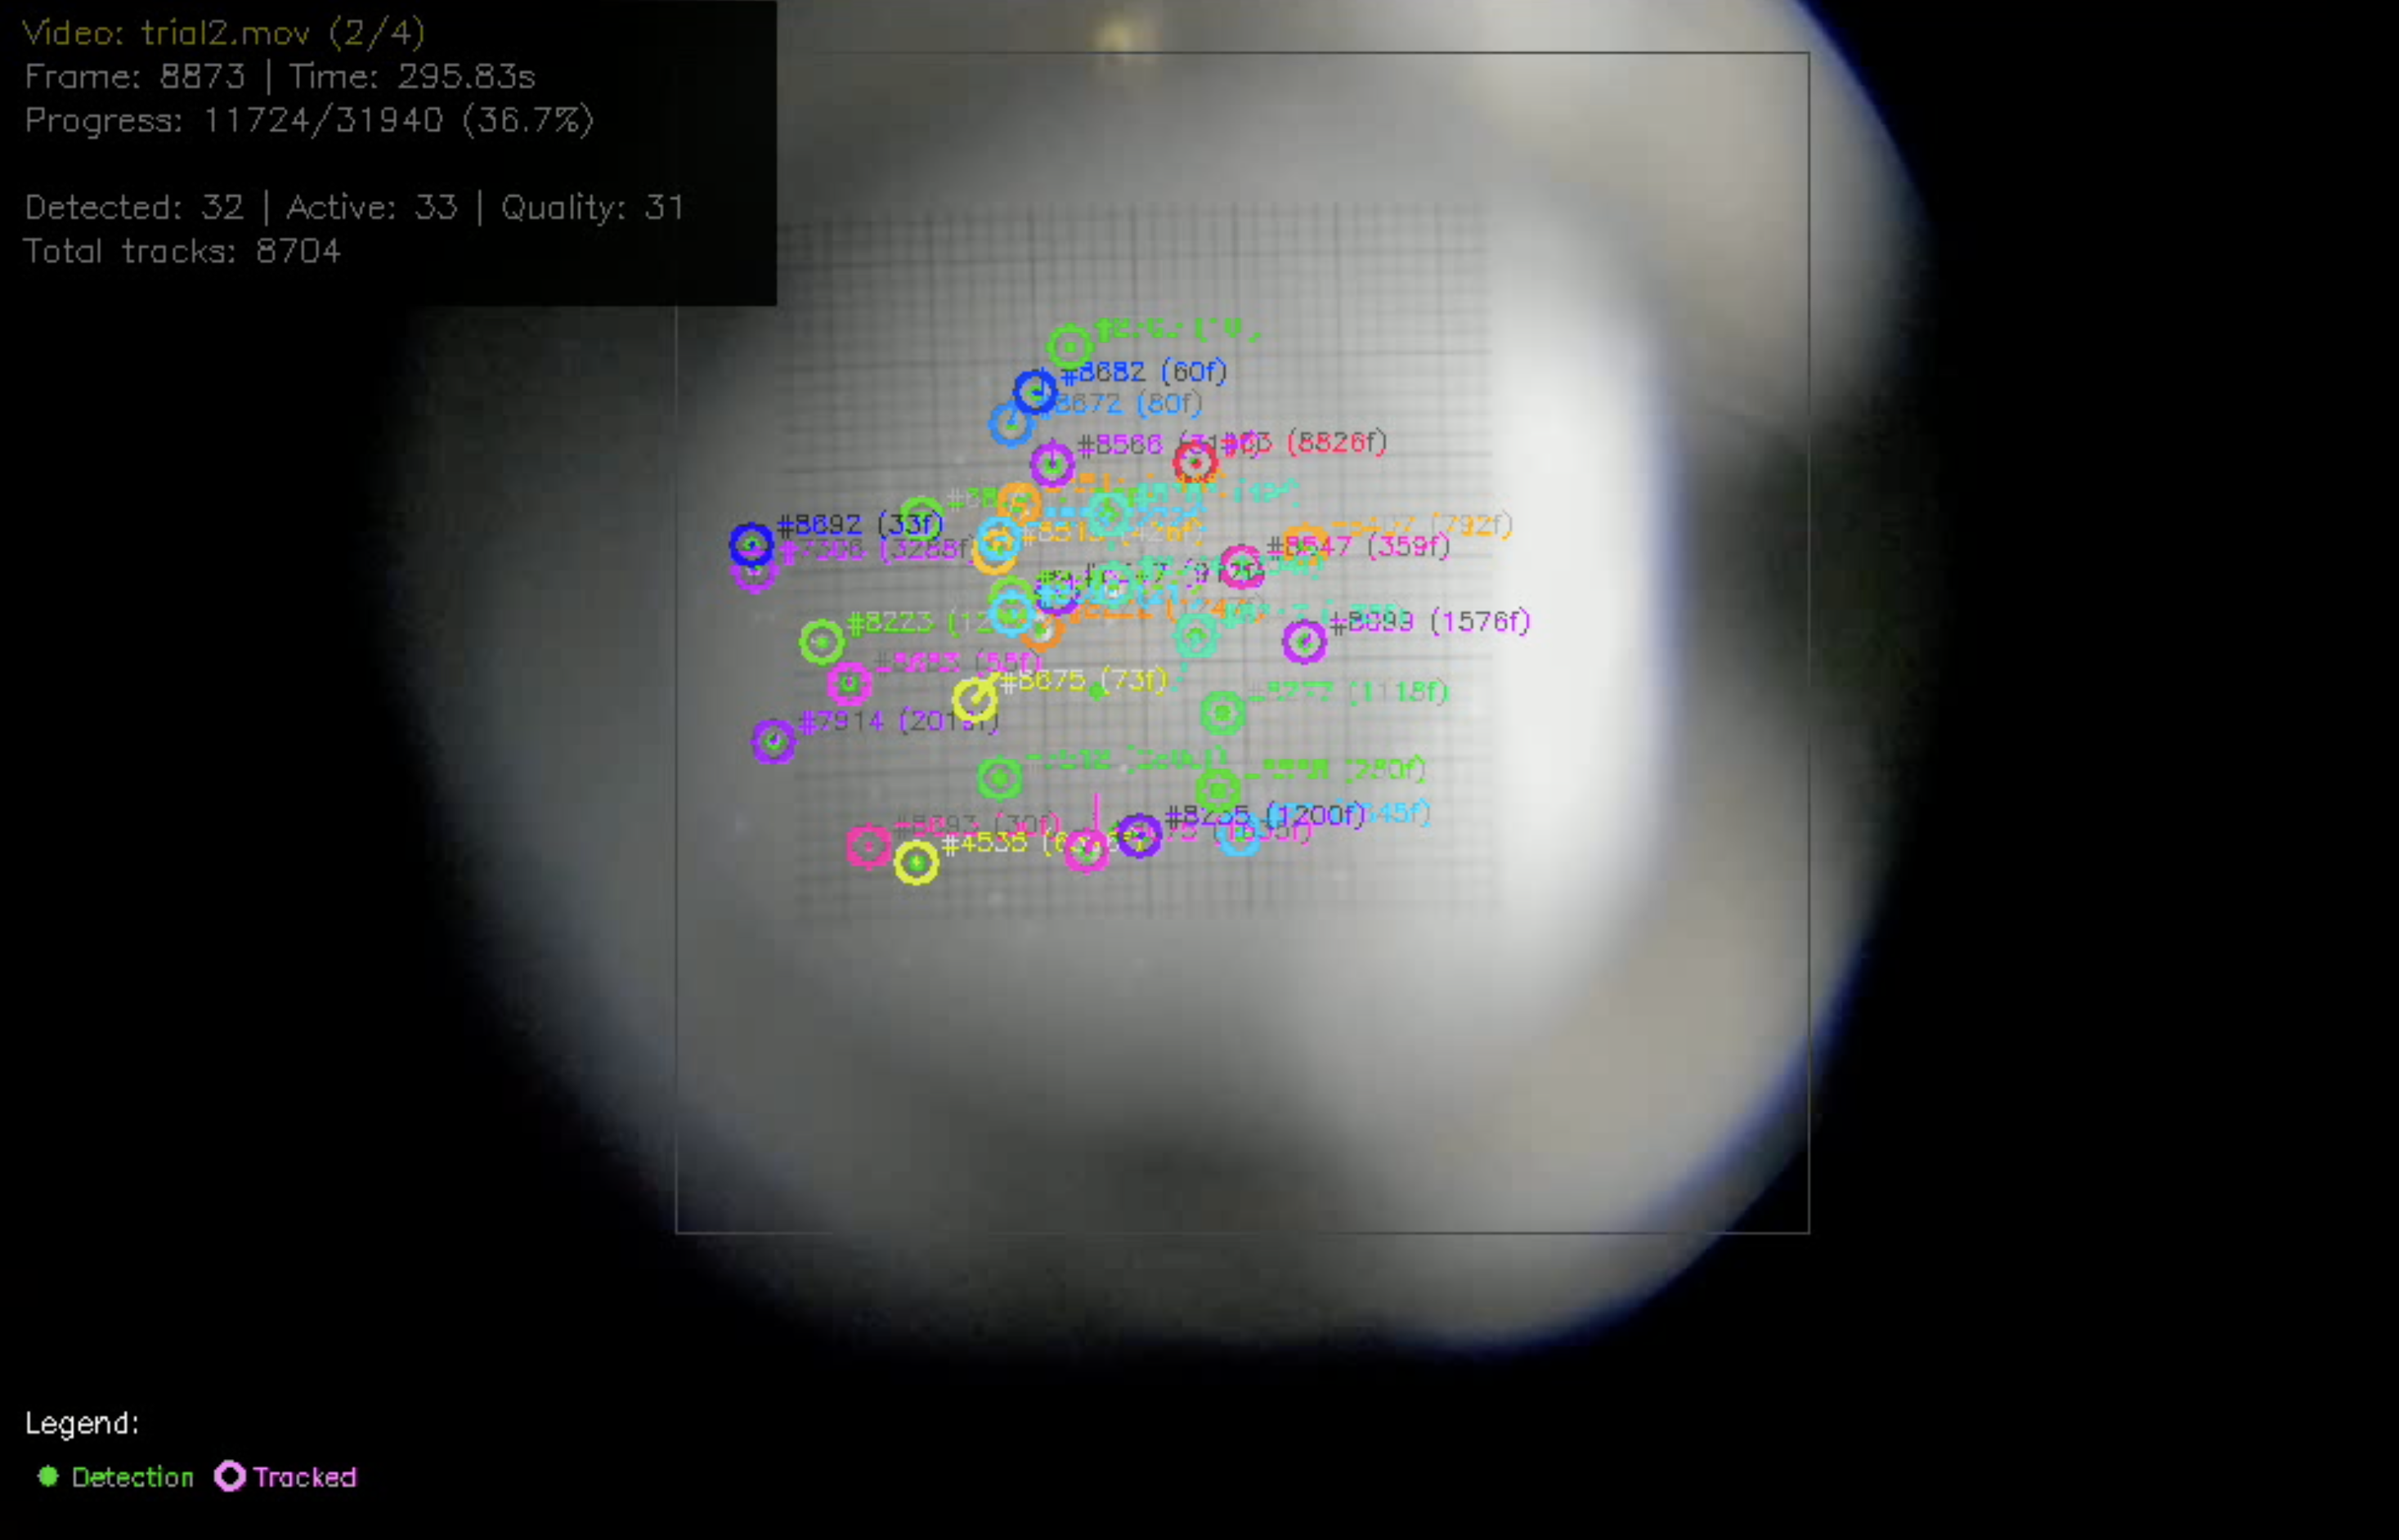
\includegraphics[width=\columnwidth]{IMG_1271.png}
\caption{Single frame from a trial video showing the computer vision tracking overlay. Detected oil droplets appear as bright spots against the dark background of the viewing chamber. Colored bounding boxes and track identifiers are drawn around each actively tracked droplet. The horizontal gridlines of the calibrated reticle (0.5~mm major spacing) are visible and used for pixel-to-millimeter calibration.}
\end{figure}


The viewing chamber contains a calibrated reticle with major gridlines spaced 0.5~mm apart and minor gridlines at 0.1~mm intervals. Automatic detection of horizontal gridlines using edge detection (Canny) and the Hough transform establishes the pixel-to-millimeter conversion factor, yielding approximately 20~pixels per millimeter for our apparatus. This calibration enables conversion of tracked pixel positions to physical velocities in mm/s.


\subsection{Calculation of the Elementary Charge}

The calculation of the elementary charge is obtained from equations (1) and (2), with the rise and fall velocities extracted for each drop. Although the charge formula contains the unitless velocity ratio $(v_f + v_r)/v_f$, the droplet radius $a$ in equation (1) depends on $v_f$ alone (not a ratio) through Stokes' law, and $a^3$ enters the charge formula. Therefore, velocities must be in physical units (m/s). The computer vision algorithm extracts velocities in pixels per second, which are converted to mm/s using the reticle calibration ($\sim$20~px/mm), and subsequently to m/s for the charge calculation. This calibration is performed automatically by detecting the reticle gridlines in the first video frame.

\subsection{Error Propagation}

Uncertainties in the calculated charge were propagated numerically: each input parameter was perturbed by $\pm$ its uncertainty, the resulting change in $q$ was computed, and individual contributions were summed in quadrature to yield the total uncertainty $\delta q$. The uncertainty in $e_{\text{calc}} = q/n$ is $\delta e = \delta q / n$. A 5\% relative uncertainty was assigned to the CV-extracted velocities, accounting for pixel calibration accuracy and centroid measurement noise. The error budget (fraction of total $\delta q^2$) is dominated by fall velocity (69\%), rise velocity (25\%), and plate separation (5\%), with all other parameters contributing less than 1\% combined.

\subsection{Computational Simulation}

The variables used in the simulation are detailed in the PASCO manual and include parameters such as voltage, plate separation, fall and rise velocities, among others. All parameters are determined experimentally, with rise and fall velocities measured repeatedly for a series of droplets, forming the bulk of the measurements. To simulate the data computationally, the fall and rise velocities are smeared using Gaussian noise, and the number of charges on each droplet is drawn from a uniform integer distribution between 1 and 9 (typical for PASCO equipment).

The experiment involves determining the charge \(Q\) on a single droplet, given by:
\[
n q_e = Q = \frac{6 \pi d}{V} \sqrt{ \frac{9 \eta^3}{2 g \rho \left(1 + \frac{b}{p a}\right)^3} } \left( v_{\text{fall}} + v_{\text{rise}} \right) \sqrt{v_{\text{fall}}}
\]

The default values for the key parameters are as follows:

\begin{table}[h]
\centering
\begin{tabular}{|l|l|}
\hline
\textbf{Variable name} & \textbf{Default value} \\
\hline
$V$ -- Voltage [V] & $500.0 \pm 0.1$ \\
\hline
$d$ -- Capacitor separation [m] & $(7.5 \pm 0.1) \times 10^{-3}$ \\
\hline
$\eta$ -- Viscosity of air [N$\cdot$s/m$^2$] & $(1.813 \pm 0.004) \times 10^{-5}$ \\
\hline
$p$ -- Barometric pressure [Pa] & $(1.01325 \pm 0.01) \times 10^{5}$ \\
\hline
$\rho$ -- Density of oil [kg/m$^3$] & $886 \pm 5$ \\
\hline
$q_e$ -- Elementary charge [C] & $1.602 \times 10^{-19}$ (accepted) \\
\hline
$b$ -- Cunningham constant [Pa$\cdot$m] & $(8.20 \pm 0.08) \times 10^{-3}$ \\
\hline
$g$ -- Gravitational acceleration [m/s$^2$] & $9.81 \pm 0.001$ \\
\hline
\end{tabular}
\caption{Physical constants and experimental parameters used in both the simulation and the physical experiment.}
\label{tab:params}
\end{table}

The simulated dataset was generated as follows. Ten individual droplets were defined, each with a fall time through 0.5~mm (the reticle spacing) drawn from the range 9.5--20.5~s and an integer charge drawn from a uniform distribution between 1 and 10. The fall time determines the droplet radius through Stokes' law and is independent of the charge. For each droplet, the rise and fall velocities were computed by inverting the governing equation, producing 10 ``perfect'' data points. Each perfect data point was then smeared 10 times with Gaussian noise at 10\% relative uncertainty, yielding 100 total simulated measurements. The same charge-extraction analysis used for the physical data was then applied to the simulated dataset; because the input \(q_e\) is known exactly, this serves as an end-to-end validation of the analysis pipeline and error propagation.
\section{Results}
\subsection{Computational Simulation}

The computational simulation was performed to generate simulated data for 10 droplets, with 10 measurements each, resulting in 100 total data points. The fall and rise velocities were smeared with Gaussian noise corresponding to a 10\% relative uncertainty to mimic experimental conditions.

The analysis procedure was applied to estimate the elementary charge from the simulated dataset. The overall estimated value is $1.6095 \times 10^{-19}$ C with a standard error of the mean of $1.7900 \times 10^{-21}$ C. This yields a relative error of 0.03\% compared to the input value of $1.609 \times 10^{-19}$ C.

Table \ref{tab:per_drop_sim} summarizes the mean and standard deviation of the estimated elementary charge for each droplet.

\begin{table}[h]
\centering
\begin{tabular}{|c|c|c|c|}
\hline
\textbf{Drop ID} & \textbf{Mean $q$ ($\times 10^{-19}$ C)} & \textbf{Std ($ \times 10^{-19}$ C)} & \textbf{Count} \\
\hline
1 & 1.59 & 0.144 & 10 \\
2 & 1.57 & 0.172 & 10 \\
3 & 1.60 & 0.170 & 10 \\
4 & 1.58 & 0.205 & 10 \\
5 & 1.61 & 0.150 & 10 \\
6 & 1.65 & 0.269 & 10 \\
7 & 1.67 & 0.255 & 10 \\
8 & 1.69 & 0.212 & 10 \\
9 & 1.58 & 0.182 & 10 \\
10 & 1.68 & 0.120 & 10 \\
\hline
\end{tabular}
\caption{Per-droplet statistics for the estimated elementary charge from the simulated data.}
\label{tab:per_drop_sim}
\end{table}

\subsection{Physical Experiment}
The physical experiment processed four trial videos comprising thousands of tracked droplet candidates. After applying validity criteria---requiring the estimated number of electrons to be between 1 and 20 and the relative error to be less than 50\%---141 valid measurements were obtained across all trials.

The distribution of the integer number of electrons ($n$) for these valid droplets is summarized in Table~\ref{tab:electron_dist}. The distribution spans broadly from $n = 2$ to $n = 20$, with measurements represented across the full range of charge states, consistent with the quantization of electric charge.

\begin{table}[h]
\centering
\begin{tabular}{|c|c||c|c||c|c|}
\hline
\textbf{$n$} & \textbf{Count} & \textbf{$n$} & \textbf{Count} & \textbf{$n$} & \textbf{Count} \\
\hline
2  & 1  & 9  & 12 & 16 & 9  \\
3  & 1  & 10 & 12 & 17 & 7  \\
4  & 5  & 11 & 9  & 18 & 10 \\
5  & 6  & 12 & 7  & 19 & 11 \\
6  & 7  & 13 & 9  & 20 & 3  \\
7  & 9  & 14 & 7  &    &    \\
8  & 3  & 15 & 13 &    &    \\
\hline
\end{tabular}
\caption{Distribution of the integer number of electrons $n$ for the 141 valid droplet measurements.}
\label{tab:electron_dist}
\end{table}

\begin{figure}[h]
\centering
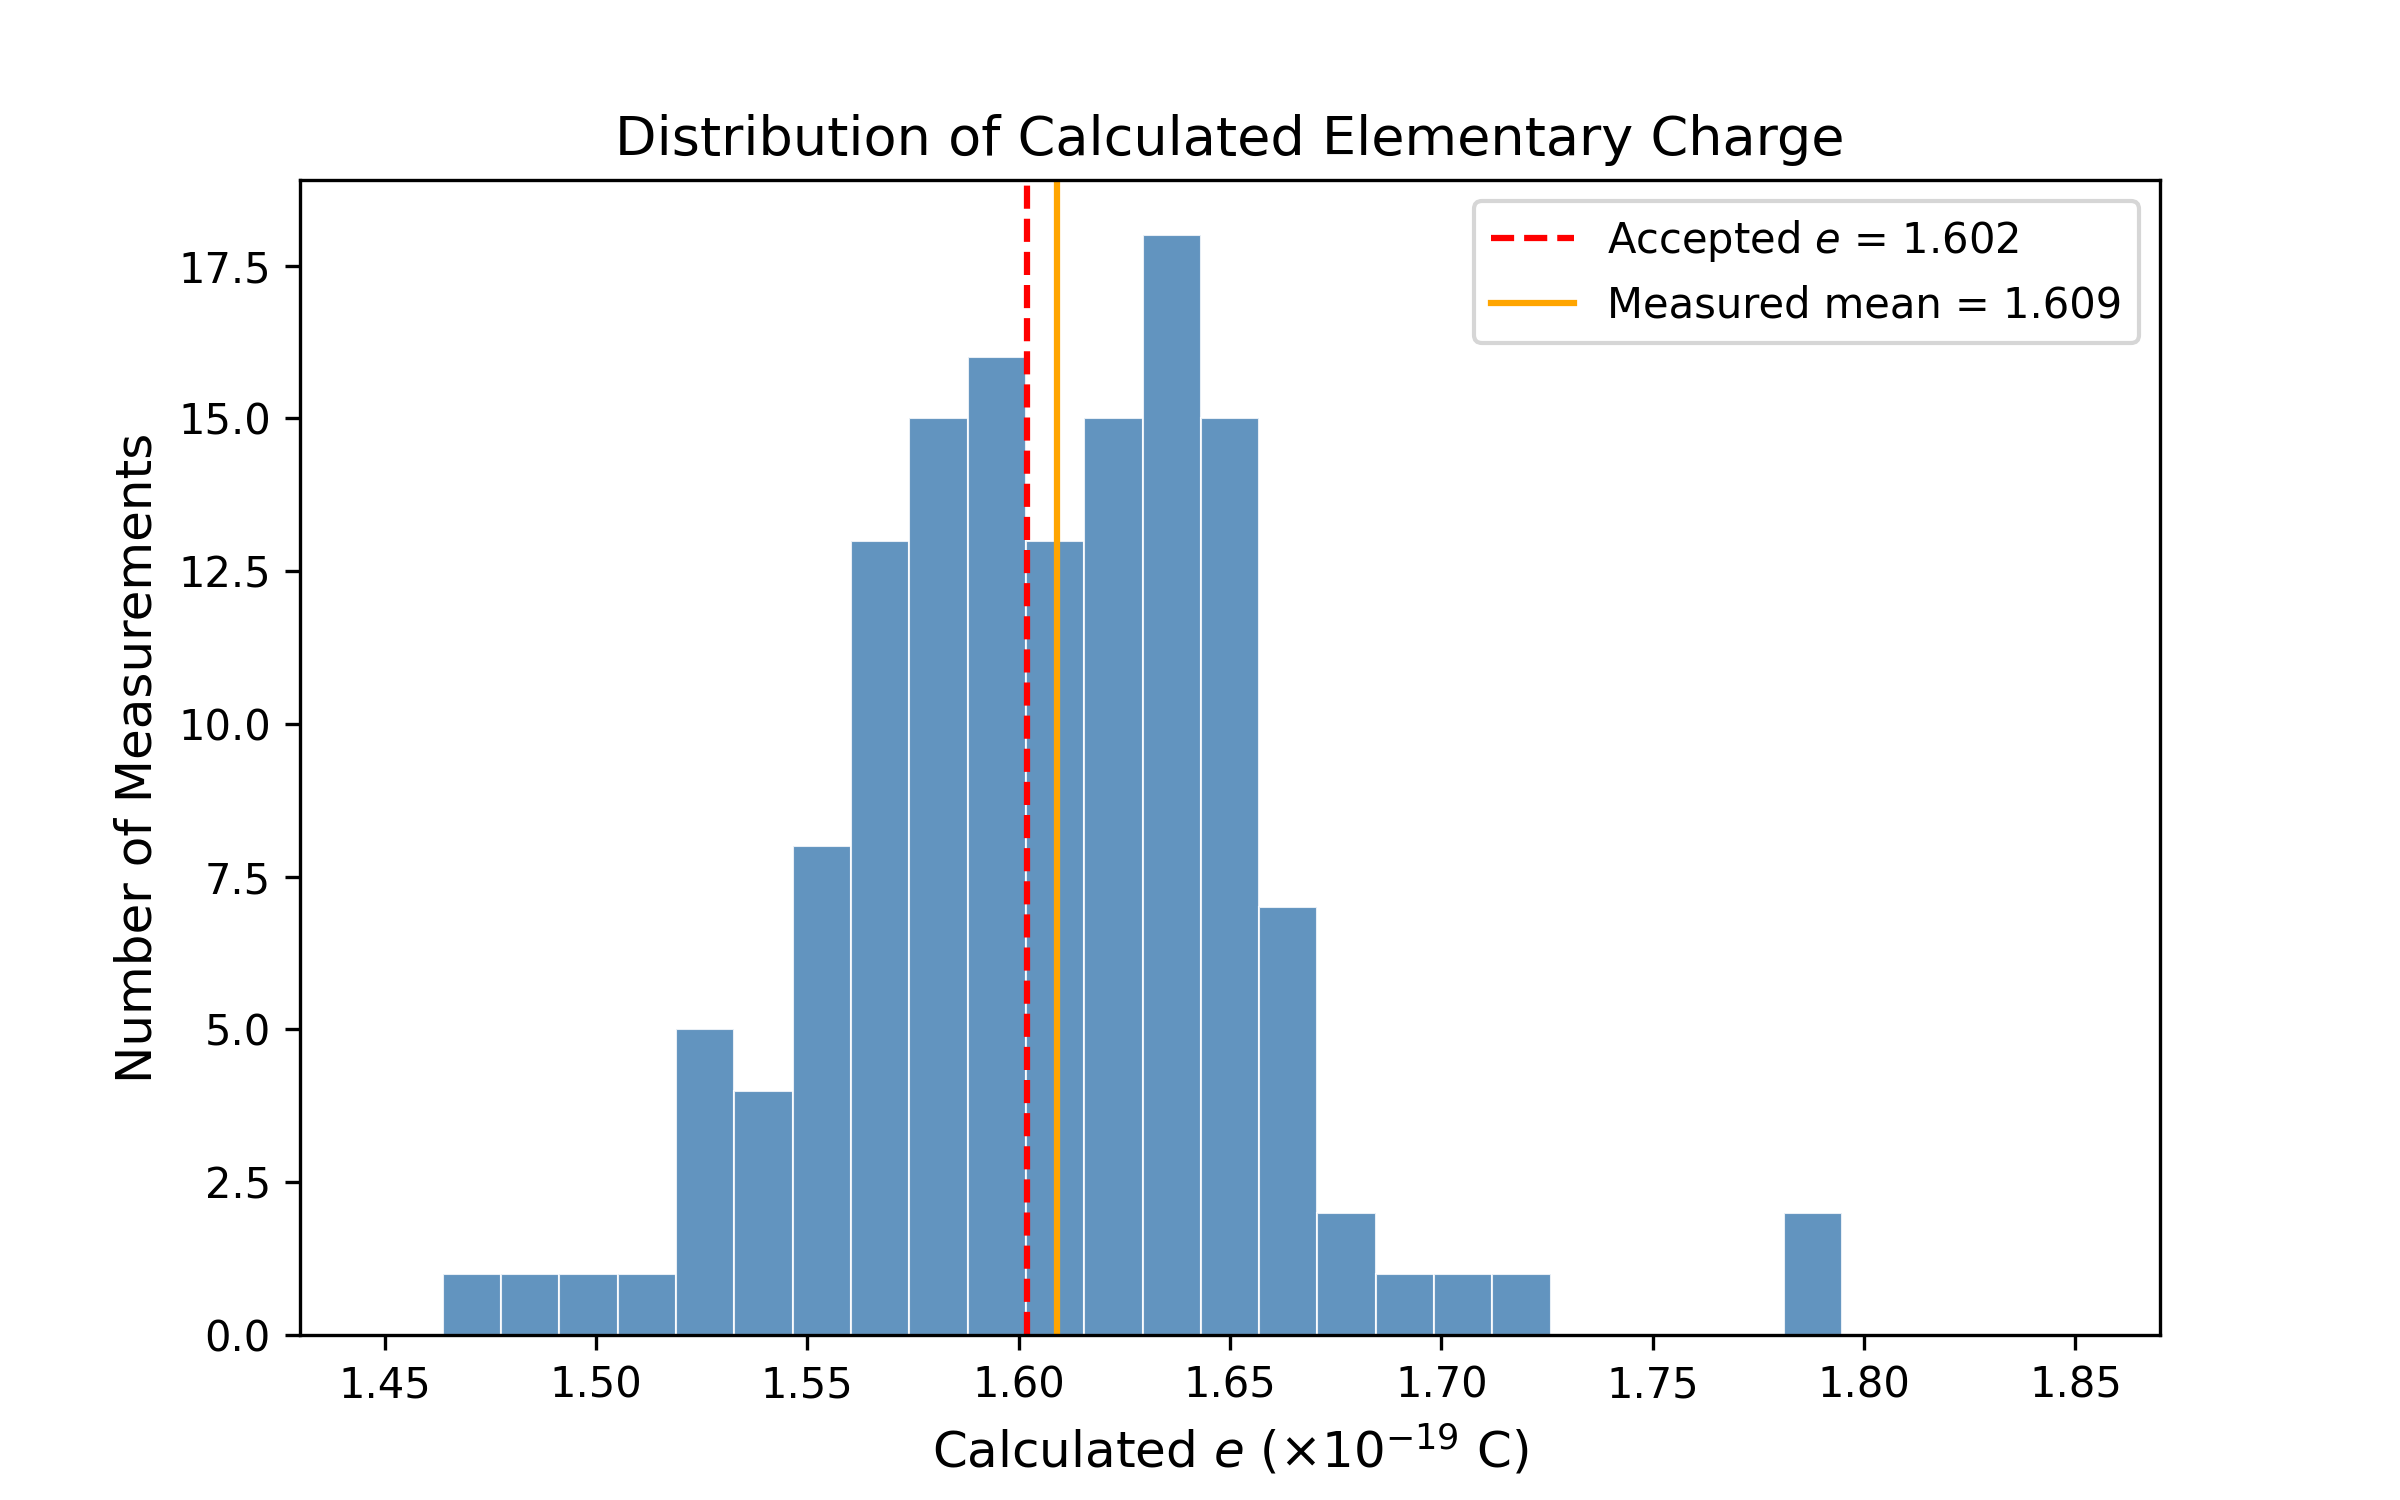
\includegraphics[width=\columnwidth]{histogram_elementary_charge.png}
\caption{Histogram of the per-measurement elementary charge estimates $e_{\text{calc}} = q/n$ for the 141 valid physical measurements. The dashed vertical line marks the accepted CODATA value $e = 1.602 \times 10^{-19}$~C. The distribution is approximately symmetric about the mean of $1.608 \times 10^{-19}$~C, with 90.1\% of measurements falling within 5\% of the accepted value.}
\end{figure}

Table~\ref{tab:trial_results} summarizes the results by trial video.

\begin{table}[h]
\centering
\begin{tabular}{|l|c|c|c|}
\hline
\textbf{Trial} & \textbf{Valid $N$} & \textbf{Mean $e_{\text{calc}}$ ($\times 10^{-19}$ C)} & \textbf{Mean Error} \\
\hline
Trial 1 & 5  & 1.618 & +0.98\% \\
Trial 2 & 65 & 1.607 & +0.33\% \\
Trial 3 & 56 & 1.608 & +0.37\% \\
Trial 4 & 15 & 1.610 & +0.48\% \\
\hline
\textbf{Total} & \textbf{141} & \textbf{1.608} & \textbf{+0.38\%} \\
\hline
\end{tabular}
\caption{Per-trial summary of elementary charge measurements.}
\label{tab:trial_results}
\end{table}

The elementary charge was estimated from these 141 valid measurements. The mean estimated value is $1.608 \times 10^{-19}$~C with a standard deviation of $5.38 \times 10^{-21}$~C and a standard error of the mean of $4.5 \times 10^{-22}$~C. The minimum and maximum individual estimates were $1.449 \times 10^{-19}$~C and $1.929 \times 10^{-19}$~C, respectively. Compared to the accepted value of $1.602 \times 10^{-19}$~C, the mean yields a percent error of +0.38\%. Of the 141 measurements, 76.6\% fall within 3\% and 90.1\% within 5\% of the accepted value. Only one measurement (trial~2, track~2343, $n = 2$) exceeds 10\% error, attributable to the very low electron count where measurement noise has the greatest relative impact.

The propagated per-measurement uncertainty $\delta e_{\text{calc}}$ averages $9.6 \times 10^{-21}$~C ($\sim$6\% relative); the breakdown by source is discussed in the following section.


\subsection{Discussion and Conclusions}

The simulation recovered \(q_e = 1.6095 \times 10^{-19}\)~C from 100 noisy measurements, deviating from the known input value by only 0.03\%. The per-droplet means in Table~\ref{tab:per_drop_sim} scatter between \(1.57\) and \(1.69 \times 10^{-19}\)~C, consistent with the 10\% Gaussian smearing applied to the velocities. This confirms that the integer-rounding charge assignment and the subsequent averaging procedure correctly extract \(q_e\) even in the presence of substantial measurement noise.

The physical experiment yielded \(q_e = (1.608 \pm 0.005) \times 10^{-19}\)~C from 141 valid measurements, a +0.38\% deviation from the 2022 CODATA value of \(1.602\,176\,634 \times 10^{-19}\)~C~\cite{NIST-e-2022}. This deviation is only $\sim$1.4 standard errors of the mean from zero, so our result is statistically consistent with the accepted value. The automated tracking far exceeded the targeted 10\% precision, largely because it produced two orders of magnitude more measurements than a manual approach would. The distribution of integer electron counts spans $n = 2$ to $n = 20$ (Table~\ref{tab:electron_dist}), confirming that the tracker captures droplets across a wide range of charge states.

Both the simulation and the experiment show a small positive bias in the mean (+0.03\% and +0.38\%, respectively). Possible sources include approximations in the Cunningham slip correction at small droplet radii and a slight systematic overestimate of the pixel-to-millimeter calibration factor, which would inflate both \(v_f\) and \(v_r\). The error budget is dominated by the fall velocity uncertainty (69\% of the total variance in $q$), followed by the rise velocity (25\%) and the plate separation (5\%); all other parameters contribute less than 1\% combined. This makes sense physically: the droplet radius depends on $v_f^{1/2}$ and enters the charge formula as $a^3$, so small errors in $v_f$ are amplified.

The main advantages of the computer vision approach over manual timing are the much larger dataset, elimination of human reaction-time error, the ability to track multiple droplets simultaneously, and full reproducibility from permanent video records. The main limitations are dependence on video quality---Trial~1 yielded only 5 valid measurements due to a shorter recording---and the pixel-to-millimeter calibration, which is the single largest source of velocity uncertainty. Since the fall velocity contributes 69\% of the total variance, doubling the camera resolution from $\sim$20~px/mm to $\sim$40~px/mm would halve the pixel quantization error in $v_f$, reducing the dominant error contribution by roughly a factor of four and lowering the overall per-measurement uncertainty from $\sim$6\% to an estimated $\sim$3\%.

In summary, using automated computer vision tracking we measured the elementary charge to be $q_e = (1.608 \pm 0.005) \times 10^{-19}$~C from 141 independent measurements, a +0.38\% deviation from the accepted CODATA value~\cite{NIST-e-2022}---well within statistical uncertainty and far exceeding the 10\% target precision. A Monte Carlo simulation of the experiment validated the analysis pipeline, recovering the input charge to within 0.03\%. The broad distribution of observed electron counts ($n = 2$ to $20$) provides direct evidence for the quantization of electric charge.

\bibliography{apssamp}% Produces the bibliography via BibTeX.

\end{document}
%
% ****** End of file apssamp.tex ******
